\documentclass[letter,11pt]{article}

\usepackage[spanish,es-nodecimaldot]{babel}
\usepackage[utf8]{inputenc}

\usepackage{lmodern}
\usepackage[T1]{fontenc}
\usepackage{textcomp}

\usepackage{framed}
\usepackage[svgnames]{xcolor}
\colorlet{shadecolor}{Gainsboro!50}

\usepackage[shortlabels]{enumitem}
\usepackage{graphicx}
\usepackage{pstricks}
\usepackage{amsmath}

\usepackage{anysize}
\marginsize{3cm}{2cm}{2cm}{3cm}

\usepackage{fancyhdr}
\usepackage{lastpage}
\pagestyle{fancy}
\fancyhf{}
\fancyhead[LE,RO]{Física Básica II}
\fancyfoot[CO,CE]{\thepage\ de \pageref{LastPage}}

\special{papersize=215.9mm,279.4mm}

\usepackage[
    pdfauthor={Carlos Eduardo Caballero Burgoa},%
    pdftitle={Física Básica II},%
    pdfsubject={Tarea 20},%
    colorlinks,%
    citecolor=black,%
    filecolor=black,%
    linkcolor=black,%
    urlcolor=black,
    breaklinks]{hyperref}
\usepackage{breakurl}

\newcommand{\blankpage}{
\newpage
\thispagestyle{empty}
\mbox{}
\newpage
}

\renewcommand{\arraystretch}{1.2}

\begin{document}

\begin{center}
    {\Large \bf{Tarea \#20}}
\end{center}

Calcular el momento de inercia de una placa rectangular uniforme respecto a un
eje principal que pasa por su centro de masa ($cm$) y es perpendicular al plano
que forma.
\\

\begin{figure}[!h]
\centering
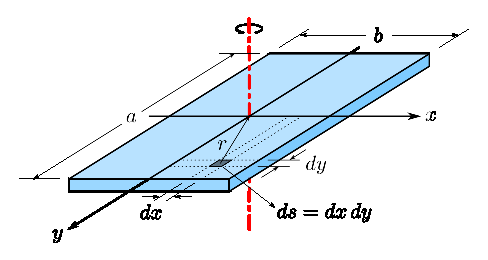
\includegraphics[scale=1.10]{resources/f1.eps}
\end{figure}

\textbf{Solución:} \\

Dada la ecuación del momento de inercia:

\begin{equation}
    I = \int_{M} r^2\, dm
\label{momentodeinercia}
\end{equation}

Siendo $r$ la hipotenusa de $x$ y $y$, por tanto:

\begin{equation}
    r^2 = x^2 + y^2
\label{pitagoras}
\end{equation}

Asumiendo la distribución homogénea de la masa:
\begin{equation*}
    \sigma = \frac{dm}{ds}
\label{densidad}
\end{equation*}

Por tanto:
\begin{equation}
    dm = \sigma\, ds = \sigma\, dx\, dy
\label{dm}
\end{equation}

Reemplazando (\ref{dm}) en (\ref{momentodeinercia}):
\begin{equation*}
    I = \int_{S} r^2\, \sigma\, ds = \int_{-a/2}^{a/2} \int_{-b/2}^{b/2} (x^2 + y^2)\, \sigma\, dx\, dy = \sigma\, \int_{-a/2}^{a/2} \left( \int_{-b/2}^{b/2} (x^2 + y^2)\, dx \right) \, dy
\end{equation*}
\begin{equation*}
    I = \sigma\, \int_{-a/2}^{a/2} \left( \int_{-b/2}^{b/2} x^2 dx + \int_{-b/2}^{b/2} y^2 dx \right) \, dy = \sigma\, \int_{-a/2}^{a/2} \left( \frac{x^3}{3} \Biggr|_{-b/2}^{b/2} + y^2 x \Biggr|_{-b/2}^{b/2} \right) \, dy
\end{equation*}
\begin{equation*}
    I = \sigma\, \int_{-a/2}^{a/2} \left( \frac{(\frac{b}{2})^3}{3} - \frac{(-\frac{b}{2})^3}{3} + y^2 \left( \frac{b}{2}\right) - y^2 \left( -\frac{b}{2}\right) \right) \, dy = \sigma\, \int_{-a/2}^{a/2} \left( \frac{b^3}{12} + b\, y^2  \right) \, dy
\end{equation*}
\begin{equation*}
    I = \sigma\, \int_{-a/2}^{a/2} \frac{b^3}{12}\, dy + \int_{-a/2}^{a/2} b\, y^2\, dy = \sigma\, \left( \frac{b^3}{12}\, y \Biggr|_{-a/2}^{a/2} + b\, \frac{y^3}{3} \Biggr|_{-a/2}^{a/2} \right)
\end{equation*}
\begin{equation*}
    I = \sigma\, \left( \frac{b^3}{12}\, \left( \frac{a}{2} + \frac{a}{2} \right) + b\, \left( \frac{(\frac{a}{2})^3}{3} - \frac{(-\frac{a}{2})^3}{3} \right) \right) = \sigma\, \left( \frac{a\, b^3}{12} + \frac{a^3\, b}{12} \right)
\end{equation*}
\begin{equation}
    I = \frac{\sigma}{12} (a\, b^3 + a^3\, b)
\label{resultado}
\end{equation}

A partir de la ecuación (\ref{dm}) sabemos que:
\begin{equation*}
    M = \sigma\, s = \sigma\, a\, b
\end{equation*}

Despejando $\sigma$ y reemplazando en la ecuación (\ref{resultado}), obtenemos:

\begin{equation*}
    I = \frac{1}{12} \left( \frac{M}{a\, b} \right) (a\, b^3 + a^3\, b) = \frac{M}{12} \left( \frac{a\, b^3}{a\, b} + \frac{a^3\, b}{a\, b} \right)
\end{equation*}

Resultando finalmente:

\begin{equation}
    I = \frac{M}{12} (a^2 + b^2)
\label{final}
\end{equation}

\end{document}

